\section{SIMULATION EXPERIMENTS}
\label{sec:expts}
\subsection{Implementation}
We compare the performance of 1SPSA-2R, 1SPSA-2H and 1RDSA-2C in the case of 
2 simulation algorithms. In the case of 1 simulation algorithms we compare the 
performance 1SPSA-1R, 1SPSA-1H and 1RDSA-1C . 
We chose i.i.d Bernoulli $\pm 1$-valued perturbations for 1SPSA-2R and 1SPSA-1R.
\footnote{The implementation is available at 
\url{https://github.com/****/1CPSA-M/archive/master.zip}.}.

For the empirical evaluations, 
we use the following two loss functions in $p=10$ dimensions:
\paragraph{Quadratic loss}
\begin{align}
J(\theta) = \theta\tr A \theta + b\tr \theta. \label{eq:quadratic}
\end{align} 
For this particular choice of $p$ the optimum $\theta^*$ for the above $J$ is 
a $10 \times 1$ column vector with each entry equal to 
$-0.9091$, and $J(\theta^*) = -4.55$.

\paragraph{Fourth-order loss}
\begin{align} 
J(\theta) = \theta \tr A\tr A\theta+0.1 \sum_{j=1}^N (A\theta)^3_j+0.01 \sum_{j=1}^N (A\theta)^4_j.\label{eq:4thorder}
 \end{align} 
The optimum $\theta^*$ for above $J$ is $\theta^*=0$, with $J(\theta^*) = 0$. 

In both functions, $A$ is such that $pA$ is an upper triangular matrix with each 
nonzero entry equal to one, $b$ is the $N$-dimensional vector of ones and 
the noise structure is similar to that used in \cite{spall_adaptive}. 
For any $\theta$, the noise is $[\theta\tr, 1]z$, where $z \approx \N(0,\sigma^2 I_{11\times11})$.
We perform experiments for noisy as well as noise-less settings, with $\sigma=0.01$ for
the noisy case. 
For all algorithms, we chose step sizes to have the form 
$\delta_n = c/(n+1)^{\gamma}$ and $a_n = 1/(n+A+1)^{\alpha}$.
We set $\alpha=0.602$ and $\gamma=0.101$.
These values for $\alpha$ and $\gamma$ have been used  before (see 
\cite{spall_adaptive}) and have demonstrated good finite-sample performance 
empirically, while satisfying the theoretical requirements needed for asymptotic 
convergence.  For all the algorithms, the initial point $\theta_0$ is the 
$p$-dimensional vector of ones.
\subsection{Results}
We use Normalized Mean Square Error (NMSE) as performance metric for evaluating 
the algorithms. 
NMSE is the ratio $\l \theta_{n_\text{end}} - \theta^* \r^2 / \l \theta_0 - \theta^*\r^2$. 
Here $n_\text{end}$ denotes the iteration number at the end of simulation budget. 

%%%%%%%%%%%%%%%%%%%%%%%%% 2 simulation NMSE results for quadratic
\begin{table}
\centering
 \caption{NMSE values of $2$ simulation methods for quadratic objective
 \eqref{eq:quadratic} with and without noise for 2000 simulations: standard error 
 from $100$ replications shown after $\pm$ symbol}
\label{tab:NMSE-quadratic}
\begin{tabular}{|c|c|}
\toprule
\rowcolor{gray!20}
\multicolumn{2}{||c|}{\multirow{2}{*}{\textbf{Noise parameter $\sigma=0.01$}}}\\[1em]
\midrule
\multirow{1}{*}{ \textbf{Method}} & \textbf{NMSE} \\
\midrule

\textbf{1SPSA-2R} & $5.762 \times 10^{-3} \pm 2.473 \times 10^{-3}$ \\
&\\
\textbf{1SPSA-2H} &$4.012 \times 10^{-5} \pm 1.654 \times 10^{-5}$\\ 
&\\
\textbf{1RDSA-2C}& $2.188 \times 10^{-5} \pm 9.908 \times 10^{-6}$\\
 \bottomrule

 
\rowcolor{gray!20}
\multicolumn{2}{||c|}{\multirow{2}{*}{\textbf{Noise parameter $\sigma=0$}}}\\[1em]
\midrule
\multirow{1}{*}{ \textbf{Method}} & \textbf{NMSE} \\
\midrule

\textbf{1SPSA-2R} & $5.755 \times 10^{-3} \pm 2.460 \times 10^{-3}$ \\
&\\
\textbf{1SPSA-2H} &$1.601 \times 10^{-5} \pm 2.724 \times 10^{-20}$ \\ 
&\\
\textbf{1RDSA-2C}& $2.474 \times 10^{-8} \pm 1.995 \times 10^{-23}$\\
 \bottomrule
\end{tabular}
\end{table}

%%%%%%%%%%%%%%%%%%%%% 2 simulation method results for fourth order
\begin{table}
\centering
 \caption{NMSE values of $2$ simulation methods for fourth order
 objective \eqref{eq:4thorder} with and without noise for 10000 simulations: standard error 
 from $100$ replications shown after $\pm$ symbol}
\label{tab:NMSE-fourthorder}
\begin{tabular}{|c|c|}
\toprule
\rowcolor{gray!20}
\multicolumn{2}{||c|}{\multirow{2}{*}{\textbf{Noise parameter $\sigma=0.01$}}}\\[1em]
\midrule
\multirow{1}{*}{ \textbf{Method}} & \textbf{NMSE} \\
\midrule

\textbf{1SPSA-2R} & $2.762 \times 10^{-2} \pm 1.415 \times 10^{-2}$ \\
&\\
\textbf{1SPSA-2H} &$3.958 \times 10^{-3} \pm 4.227 \times 10^{-4}$\\ 
&\\
\textbf{1RDSA-2C}& $3.598 \times 10^{-3} \pm 4.158 \times 10^{-4}$\\
 \bottomrule

 
\rowcolor{gray!20}
\multicolumn{2}{||c|}{\multirow{2}{*}{\textbf{Noise parameter $\sigma=0$}}}\\[1em]

\midrule
\multirow{1}{*}{ \textbf{Method}} & \textbf{NMSE} \\
\midrule

\textbf{1SPSA-1R} & $2.747 \times 10^{-2} \pm 1.413 \times 10^{-2}$ \\
&\\
\textbf{1SPSA-1H} &$3.901 \times 10^{-3} \pm 4.359 \times 10^{-18}$ \\ 
&\\
\textbf{1RDSA-1C}& $3.535 \times 10^{-3} \pm 1.743 \times 10^{-18}$\\
 \bottomrule
\end{tabular}
\end{table}

%%%%%%%%%%%%%%%%%%%%%%%%%% 1 simulation method results for quadratic

\begin{table}
\centering
 \caption{NMSE values of $1$ simulation methods for quadratic
 objective \eqref{eq:quadratic} with and without noise for 20000 simulations: standard error 
 from $100$ replications shown after $\pm$ symbol}

\label{tab:NMSE-quadratic-1sim}
\begin{tabular}{|c|c|}
\toprule
\rowcolor{gray!20}
\multicolumn{2}{||c|}{\multirow{2}{*}{\textbf{Noise parameter $\sigma=0.01$}}}\\[1em]
\midrule
\multirow{1}{*}{ \textbf{Method}} & \textbf{NMSE} \\
\midrule

\textbf{1SPSA-1R} & $8.582 \times 10^{-2} \pm 3.691 \times 10^{-2}$ \\
&\\
\textbf{1SPSA-1H} &$2.774 \times 10^{-2} \pm 2.578 \times 10^{-4}$\\ 
&\\
\textbf{1RDSA-1C}& $8.225 \times 10^{-3} \pm 5.959 \times 10^{-5}$\\
 \bottomrule

 
\rowcolor{gray!20}
\multicolumn{2}{||c|}{\multirow{2}{*}{\textbf{Noise parameter $\sigma=0$}}}\\[1em]

\midrule
\multirow{1}{*}{ \textbf{Method}} & \textbf{NMSE} \\
\midrule

\textbf{1SPSA-1R} & $8.584 \times 10^{-2} \pm 3.681 \times 10^{-2}$ \\
&\\
\textbf{1SPSA-1H} &$2.770 \times 10^{-2} \pm 3.836 \times 10^{-17}$ \\ 
&\\
\textbf{1RDSA-1C}& $8.225 \times 10^{-3} \pm 1.569 \times 10^{-17}$\\
 \bottomrule
\end{tabular}
\end{table}



%%%%%%%%%%%%%%%%%%%%% 1 simulation method results for fourth order
\begin{table}
\centering
 \caption{NMSE values of $1$ simulation methods for fourth order
 objective \eqref{eq:4thorder} with and without noise for 20000 simulations: standard error 
 from $100$ replications shown after $\pm$ symbol}
\label{tab:NMSE-fourthorder-1sim}
\begin{tabular}{|c|c|}
\toprule
\rowcolor{gray!20}
\multicolumn{2}{||c|}{\multirow{2}{*}{\textbf{Noise parameter $\sigma=0.01$}}}\\[1em]
\midrule
\multirow{1}{*}{ \textbf{Method}} & \textbf{NMSE} \\
\midrule

\textbf{1SPSA-1R} & $3.240 \times 10^{-1} \pm 1.836 \times 10^{-1}$ \\
&\\
\textbf{1SPSA-1H} &$8.916 \times 10^{-2} \pm 1.896 \times 10^{-2}$\\ 
&\\
\textbf{1RDSA-1C}& $4.972 \times 10^{-2} \pm 9.812 \times 10^{-3}$\\
 \bottomrule

 
\rowcolor{gray!20}
\multicolumn{2}{||c|}{\multirow{2}{*}{\textbf{Noise parameter $\sigma=0$}}}\\[1em]

\midrule
\multirow{1}{*}{ \textbf{Method}} & \textbf{NMSE} \\
\midrule

\textbf{1SPSA-1R} & $3.192 \times 10^{-1} \pm 1.991 \times 10^{-1}$ \\
&\\
\textbf{1SPSA-1H} &$8.173 \times 10^{-2} \pm 1.255 \times 10^{-16}$ \\ 
&\\
\textbf{1RDSA-1C}& $4.403 \times 10^{-2} \pm 9.066 \times 10^{-17}$\\
 \bottomrule
\end{tabular}
\end{table}





\begin{figure}
\caption{$\log_{10}(\text{NMSE})$vs No of iterations for quadratic 
objective \eqref{eq:quadratic} with noise ($\sigma=0.01$) using 2 simulation methods.}
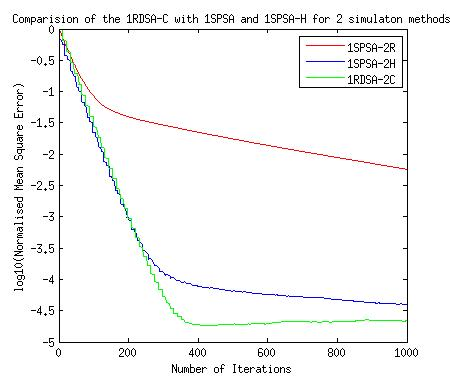
\includegraphics[width=8cm, height=7cm]{results_noise_quad.jpg}\label{fig:noise_quad}
\end{figure}

\begin{figure}
\caption{$\log_{10}(\text{NMSE})$vs No of iterations for fourth order objective 
objective \eqref{eq:4thorder} with noise ($\sigma=0.01$) using 2 simulation methods.}
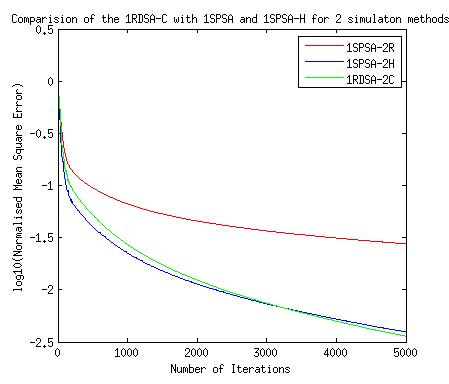
\includegraphics[width=8cm, height=7cm]{results_noise_fourthorder.jpg}\label{fig:noise_4thorder}
\end{figure}

\begin{figure}
\caption{$\log_{10}(\text{NMSE})$vs No of iterations for quadratic order objective 
objective \eqref{eq:quadratic} with noise ($\sigma=0.01$) using 1 simulation methods.}
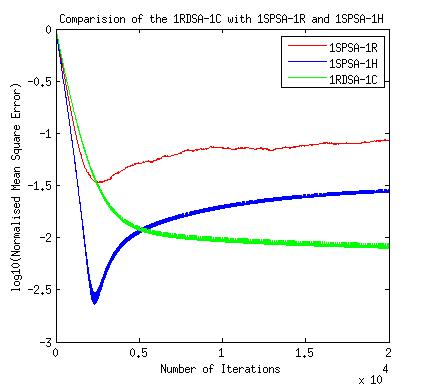
\includegraphics[width=8cm, height=7cm]{results_noise_1sim_quad.jpg}\label{fig:noise_quad_1sim}
\end{figure}

\begin{figure}
\caption{$\log_{10}(\text{NMSE})$vs No of iterations for fourth order objective 
objective \eqref{eq:4thorder} with noise ($\sigma=0.01$) using 1 simulation methods.}
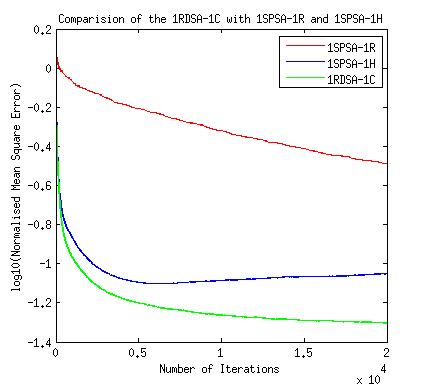
\includegraphics[width=8cm, height=7cm]{results_noise_1sim_fourthorder.jpg}\label{fig:noise_4thorder_1sim}
\end{figure}




Tables \ref{tab:NMSE-quadratic}--\ref{tab:NMSE-fourthorder} present the 
normalized mean square values observed for the three algorithms - 1SPSA-2R, 1SDSA-2H and 
1RDSA-2C for the fourth-order and quadratic loss functions respectively.
Table \ref{tab:NMSE-fourthorder-1sim}--\ref{tab:NMSE-quadratic-1sim} present 
the NMSE values observed for the three algorithms - 1SPSA-1R, 1SPSA-1H  and 1SPSA-1C
with the fourth order and quadratic loss functions respectively. 
The results  in Table \ref{tab:NMSE-quadratic} is after $2000$ simulations and
the results in Table \ref{tab:NMSE-fourthorder} is after $10000$ simulations.
The results in Table \ref{tab:NMSE-fourthorder-1sim}--\ref{tab:NMSE-quadratic-1sim} are 
obtained after running the 1 simulation algorithms with a budget of $20000$ simulations. 

Figure \ref{fig:noise_quad} and \ref{fig:noise_4thorder} plots the $\log_{10}\text{(NMSE)}$ as
a function of the iterations with quadratic and fourth-order loss objectives respectively,
with $\sigma=0.01$ 


Figure \ref{fig:noise_quad_1sim} and \ref{fig:noise_4thorder_1sim} plots the 
$\log_{10}\text{(NMSE)}$ as a function of the iterations with quadratic and fourth-order loss 
objectives respectively, with $\sigma=0.01$ 

From the results in Tables \ref{tab:NMSE-quadratic},\ref{tab:NMSE-fourthorder}
\ref{tab:NMSE-quadratic-1sim},\ref{tab:NMSE-fourthorder-1sim} and 
plots \ref{fig:noise_quad} \ref{fig:noise_4thorder} \ref{fig:noise_quad_1sim} 
\ref{fig:noise_4thorder_1sim}, we make the following observations:
 
\textit{\textbf{Observation1}} In the case of two simulation algorithms 1RDSA-2C is slightly better than 
1SPSA-2H, while both of them outperform 1SPSA-2R.

\textit{\textbf{Observation2}} In the case of one simulation algorithms 1RDSA-1C is better than both 
1SPSA-1H and 1SPSA-1R.

